\documentclass[10pt,a4paper]{article}
\usepackage[latin1]{inputenc}
%\usepackage[ngerman]{babel}
\usepackage{amsmath}
\usepackage{amsfonts}
\usepackage{amssymb}
\usepackage{graphicx}
\usepackage{multicol}
\usepackage{framed}
\usepackage{mdframed}

\newcommand{\plus}{{\;} + {\;}}
\newcommand{\minus}{{\;} - {\;}}
\renewcommand{\div}{\text{div} {\;}}
\newcommand{\grad}{\text{grad} {\;}}
\renewcommand{\d}{{\;} \text{d}}
\renewcommand{\vec}[1]{\boldsymbol{#1}}

\title{Finite Element Method}

\begin{document}

\section{Introduction}

Imagine a problem which can be expressed mathematically through the use of 
partial differential equations (PDEs). This can be for example a heat flux in 
the parts of a wind turbine (heat equation). Or it can be the description of 
the electro-magnetic behaviour of a coil in a circuit (Maxwell's equations). 
Usually these equations can be solved analytically only for fairly simplified 
cases. For more complicated problems (e.g. more complex geometries) it is 
useful to move away from the analytical formulation and discretize the system. 
Then this system can be described by a system of equations which can be solved 
numerically (i.e. by a computer). 

The Finite Element Method (FEM) is a widely used method in industry and 
academic research and makes use of the idea described above. It breaks down the 
entire system into elements and solves the resulting equations piecewise for 
each of these elements. The overall result is thereby an assembly of all 
smaller equations. Since by discretization one always can only mimic the model 
in the real world only approximately the result is also only an approach to the 
exact solution. Nevertheless, there exist methods, by which it is possible to 
come close to the exact solution. 


\section{The Three Steps of FEM}

\subsection{Preprocessing}
Before starting to calculate it is necessary to pass the software 
information to start with. These information include in general the following 
points: 

\begin{itemize}
	\item \textbf{Geometry:} Description of the form of the modelled body.
	\item \textbf{Material:} The properties of the body (Young's modulus, heat 
	conductivity, density, etc.).
	\item \textbf{Geometrical Boundary Conditions (BCs):} In which directions 
	is the model allowed to move? In which directions does it have to move?
	\item \textbf{Static BCs:} Is there a static force acting at any points?
	\item \textbf{Volume loads:} Are there any volume forces (e.g. gravity, 
	electric forces)?
	\item \textbf{Type of elements:} Defines the shape of the finite elements. 
	Usually these shapes are relatively simple (e.g. squares, triangles, 
	tetrahedrons).
	\item \textbf{Mesh generation:} The process of dividing the model into a 
	number of finite elements.
\end{itemize}

\subsubsection{Geometry}

The input of the geometry is usually done via a CAD (\textit{Computer Aided 
Design}) file which is imported into the FEM software. On the other hand one 
can 
build the desired geometry in the software itself. The more accurate the 
results shall be in the end, the more accurate of course should be the geometry 
of the model. However, often it is possible to reduce the accuracy of the model 
to a certain degree without losing to much accuracy in the results. This helps 
reducing the computational costs. 

For more complicated geometries it is convenient to introduce local coordinate 
systems in which parts can be constructed separately. This has the advantage 
that one can subdivide the different building steps into several independent 
parts which makes the building process more effective. 

\subsubsection{Material}

In this section the material parameters as well as the constitutive equations 
(CEs) are introduced. The parameters can include all possible information that 
can be connected to a material. This includes following properties


\begin{itemize}
	\item \textbf{Mechanical: } Young's modulus, Poisson ratio, shear modulus, 
	Lam� parameters, etc. 
	\item \textbf{Thermal: } Heat conductivity, specific heat, etc. 
	\item \textbf{Diffusive: } Diffusion coefficient, porosity, etc. 
	\item \textbf{Electrical: } Electrical conductivity, rel. permittivity, 
	etc. 
	\item \textbf{Magnetic: } Susceptibility, magnetic permittivity, etc.
	\item \textbf{Chemical: } Solubility, chemical resistance, etc. 
\end{itemize}

and many more. 


\subsubsection{Geometrical BCs, static BCs and volume forces}

A PDE itself has without nearer definition infinite many solutions. Also the 
system of equations after discretizing the model still has infinite many 
solutions (mathematically this is equivalent to say that the system of 
equations is \textit{linear independent}). Only after applying specific 
boundary conditions to the system it becomes \textit{linear dependent} and is 
solvable. 

In general there are three different kinds of boundary conditions. The first one is the \textit{Dirichlet boundary condition}. If the differential equation is dependent for example on the displacement this means that we prescribe the displacement of a point or line of the boundary in a specific direction. 
In contrast to that \textit{Neumann boundary conditions} prescribe the first 
spacial derivative orthogonal to the boundary. In our example this would mean 
to prescribe the force at the boundary.\textbf{ (Why the force?) }

If no boundary conditions are applied at some point, this point is stated to be 
\textit{free}. 

\subsubsection{Division of the Model in Elements}

For the sake of discretization the model is split into a finite number of 
elements, hence the name \textit{Finite Element Method}. To reduce the 
complexity of computation the elements chosen have a simple form. Since it is 
not always possible to divide the model into these kind of simple shapes, the 
elements will be mapped before the computation process to an even simpler 
shape (i.{}e. quadrilateral and equilateral triangle in 2D, and hexahedral or 
equilateral tetrahedral in 3D).

Now, that the model is divided into many parts, it consists of elements and 
nodes. During the deformation these nodes experience a displacement, which is 
given by the constraints of the whole model. The aim during the computation is 
to find out all the displacements for the nodes according to the given boundary 
conditions. 

In figure \ref{mesh} the possible element shapes are shown for 2D and 3D 
models. 

\begin{figure}
	\begin{minipage}{6cm}
		\centering
		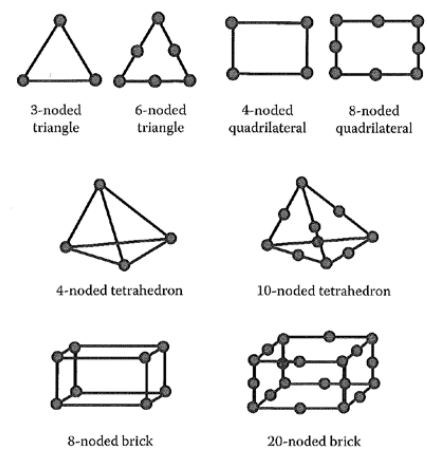
\includegraphics[width = 5cm]{element_shapes}
	\end{minipage}
	\begin{minipage}{6cm}
		\centering
		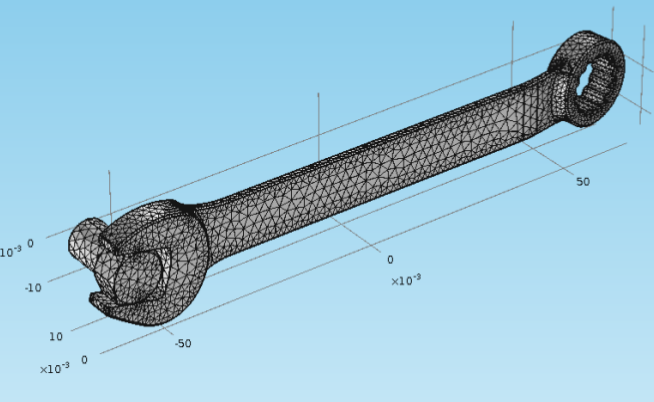
\includegraphics[width = 6cm]{3d_mesh}
	\end{minipage}
	\caption{left: Different element shapes for 2D and 3D models, right: 
	possible mesh with tetrahedrals}
	\label{mesh}
\end{figure}

The mesh generation itself can happen automatically (for complex geometries) or 
manually (for simple geometries). But one should keep in mind that in 3D an 
automatic meshing is not possible for hexahedrals or bricks but only for 
tetrahedrals. 





\subsection{Processing}

During the processing the calculation with all given constraints is performed. 
The following steps are required: 

\begin{itemize}
	\item \textbf{Calculation of the element stiffness matrices:} They describe 
	the behaviour of each element during the deformation process.
	\item \textbf{Calculation of the element load vectors:} They describe which 
	elements have constraints due to boundary conditions or which ones only 
	border on other elements.
	\item \textbf{Assembling:} The whole system is build up by the summation of 
	all elements considering how the model is split up into these ones.
	\item \textbf{Solution of the governing system of equations:} This is the 
	last step and computes all displacements for each node and so for the whole 
	model. 
\end{itemize}

\subsection{Post processing}

After the computation follows the post-processing. This also includes that the 
engineer interprets and controls the solutions of the simulation. All in all the 
following steps are necessary:

\begin{itemize}
	\item \textbf{Separation of the element displacement vectors:} Which global 
	node displacement belongs to which element?
	\item \textbf{Calculation of the approximated continuous displacements with 
	ansatz functions:} Until now we only had the displacements at the positions 
	of the nodes. This is why we also need to calculate an approximation in the 
	inner regions of the elements.
	\item \textbf{Calculation of the approximated continuous strains and 
	stresses:} e.{}g. in 1D the strain $ \varepsilon $ of a bar with the length 
	$ l $ is given 
	by:
	
	\begin{equation}
		\varepsilon(x) = \dfrac{\Delta l}{l}
	\end{equation}
	
	Furthermore the stress $ \sigma $ is given by the following equation:
	
	\begin{equation}
	\sigma(x) = E\varepsilon = E \dfrac{\Delta l}{l}
	\end{equation}
	
	In general the equations more complicated but they show 
	the idea of the post processing.
	
	\item \textbf{Visualization of deformations, strains, stresses, etc.}
	\item \textbf{Interpretation of the solutions and error analysis}
\end{itemize}

In figure \ref{example2ScrewWrench} some visualizations after the post-processing step are shown.

\begin{figure}[h]
	\centering
	\begin{minipage}{11cm}
		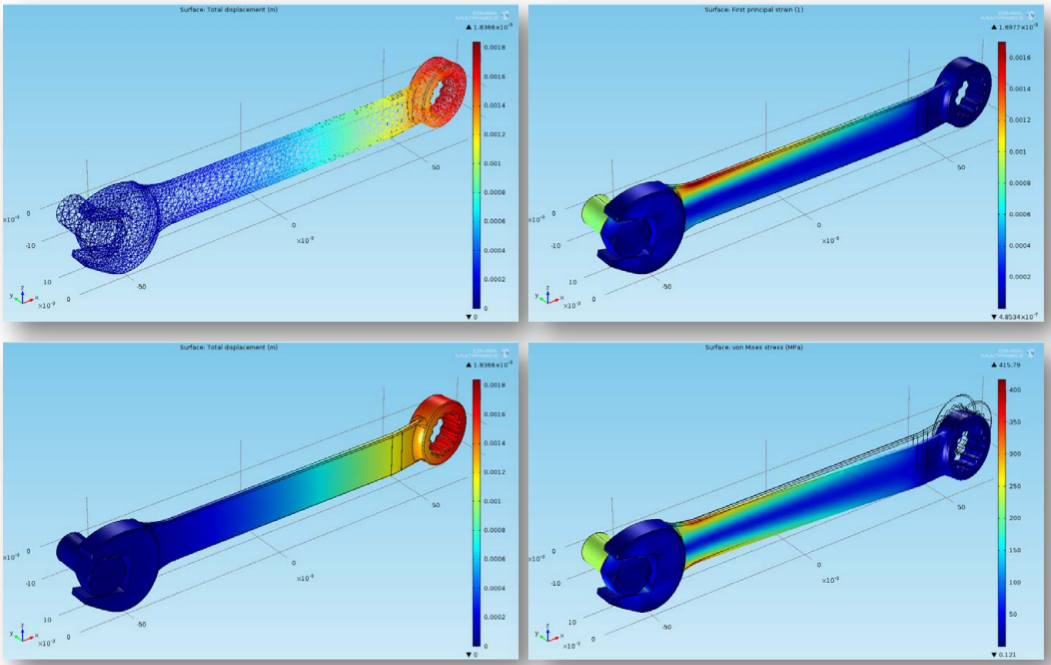
\includegraphics[width = 11cm]{example2}
	\end{minipage}
	\caption{Total displacement together with mesh (\textit{top left:}), 
	principal strain in x-direction (\textit{top right:}), total strain 
	(\textit{bottom left:}) and von-Mises stress (\textit{bottom right}) of a 
	screw wrench while setting tight a screw }
	\label{example2ScrewWrench}
\end{figure}


\pagebreak

In the following a summary of the whole FEM process is given. 

%%%%%%%%%%%%%%%%%%%%%%%%%%%%%%%%%%%%%%%%%%%%%%%%%%%%%%%%%%%%%%%%%%%%%%%
%
%    Es fehlen noch Pfeile zwischen den einzelnen K�sten
%
%%%%%%%%%%%%%%%%%%%%%%%%%%%%%%%%%%%%%%%%%%%%%%%%%%%%%%%%%%%%%%%%%%%%%%%

\begin{mdframed}
	\begin{center}
		\textbf{Model building} \\
		\text{\small Translation of the physical problem in a mathematical and 
		geometrical model;} \\
		\text{\small Formulation of the respective differential equations and 
		boundary conditions}
	\end{center} 
\end{mdframed}



\begin{mdframed}
	\begin{center}
		\textbf{Weak Formulation} \\
		\text{\small Transformation from (local) differential equations and B.C.s to (global) integral} \\
		\text{\small formulations - weak form of differential equation}
	\end{center} 
\end{mdframed}



\begin{mdframed}
	\begin{center}
		\textbf{Discretization of Geometry} \\
		\text{\small Dividing the geometry into geometrical similar parts} \\
		\text{\small and application of the weak form onto them}
	\end{center} 
\end{mdframed}



\begin{mdframed}
	\begin{center}
		\textbf{Discretization of PDEs} \\
		\text{\small Approximation of continious primary variables with ansatz} 
		\\
		\text{\small functions und discrete primary variables;} \\
		\text{\small Formulation of element matrices and load vectors}
	\end{center} 
\end{mdframed}



\begin{mdframed}
	\begin{center}
		\textbf{Assembling} \\
		\text{\small Reassembling of element matrices and element vectors to system variables;} \\
		\text{\small This leads to the discrete weak form of the system}
	\end{center} 
\end{mdframed}



\begin{mdframed}
	\begin{center}
		\textbf{Fundamental Lemma of Variational Calculus} \\
		\text{\small The weak form must be fullfilled for all primary variables of the system} \\
		\text{\small which leads to a system of equations for the discrete 
		variables}
	\end{center} 
\end{mdframed}



\begin{mdframed}
	\begin{center}
		\textbf{Solution of the System of Equations} \\
		\text{\small Direct solution for linear stationary systems} \\
		\text{\small Time integration and iterative solution f�r non-linear non-stationary systems}
	\end{center} 
\end{mdframed}



\begin{mdframed}
	\begin{center}
		\textbf{Computation of dependent Variables} \\
		\text{\small Computation of dependent variables with the solution for the discrete} \\
		\text{\small primary variables and the ansatz function on the element 
		level}
	\end{center} 
\end{mdframed}

\pagebreak

\section{Mathematical Background}

In this chapter the basic mathematical tools for an FEM simulation shall be introduced. We will concentrate in the following on the description for mechanical problems.

\subsection{Main ingredients for an FEM analysis in mechanics}

\subsubsection{Basic Variables}

At first there shall be defined the following variables:

\begin{align}
\text{displacement vector:} & \qquad \vec{u} = u_{i} \nonumber \\
\text{strain tensor:} 		& \qquad \vec{\varepsilon} = \varepsilon_{ij}  \nonumber \\
\text{stress tensor:}		& \qquad \vec{\sigma} = \sigma_{ij} \nonumber  \\
\text{material properties:}	& \qquad \mathbb{C} = C_{ijkl} \nonumber 
\end{align}

or in 1D:

\begin{align}
\text{displacement:} & \qquad \Delta l = l - l_{0} \nonumber \\
\text{strain:} 		& \qquad \varepsilon = \dfrac{l-l_{0}}{l_{0}} = 
\dfrac{\Delta l}{l_{0}}  \nonumber \\
\text{stress:}		& \qquad \sigma = \dfrac{E}{\varepsilon} = \dfrac{F}{A} 
\nonumber  \\
\text{material properties:}	& \qquad E \nonumber 
\end{align}

where the geometrical variables are declared in figure \ref{barsAndVector}.

\begin{figure}[h]
	\begin{minipage}{6cm}
		\centering
		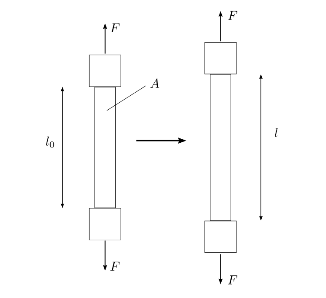
\includegraphics[width = 6cm]{elongation}
	\end{minipage}
	\begin{minipage}{6cm}
		\centering
		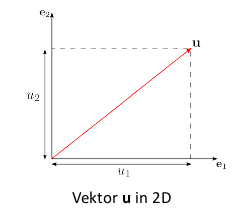
\includegraphics[width = 5cm]{2Dvector}
	\end{minipage}
	\caption{left: A 1D example of the elongation of a bar element, right: a vector in 2D}
	\label{barsAndVector}
\end{figure}

\pagebreak

\begin{framed}
\textbf{Short Summary of Vectors and Tensors} \\

A vector can be written as a linear combination of three basis vectors that span a three dimensional space. 

\begin{equation}
\vec{u} = u_{1}\vec{e}_{1} + u_{2}\vec{e}_{2} + u_{3}\vec{e}_{3} = \sum\limits_{i = 1}^{3} u_{i}\vec{e}_{i} \nonumber
\end{equation}

A vector can also be written in column notation as

\begin{equation}
\vec{u} = \begin{bmatrix} u_{1} \\ u_{2} \\ u_{3} 
\end{bmatrix} . \nonumber
\end{equation}

Tensors are "matrices with a basis", for example

\begin{equation}
\vec{\sigma} = \sigma_{ij} {\;} \vec{e}_{i} \otimes \vec{e}_{j} \nonumber
\end{equation}

\begin{equation}
\vec{\sigma} = \begin{bmatrix} \sigma_{11} & \sigma_{12} & \sigma_{13} \\ \sigma_{21} & \sigma_{22} & \sigma_{23} \\ \sigma_{31} & \sigma_{32} & \sigma_{33} 
\end{bmatrix} . \nonumber
\end{equation}
\end{framed}

\subsubsection{Basic Equations of Mechanics}

Here, the starting point is Newton's 2\textsuperscript{nd} law of mechanics:

\begin{quotation}
The alteration of motion is ever proportional to the motive force impress'd; and is made in the direction of the right line in which that force is impress'd. \footnote{from Motte, 1729}
\end{quotation}

This also can be expressed through the well known formula

\begin{equation}
F = m \cdot \vec{a} = m \cdot \ddot{x} .
\end{equation}

Furthermore, the total force $ \vec{F}_{T} $ acting on a body can be separated into two parts:

\begin{equation}
\vec{F}_{T} = \vec{F}_{B} + \vec{F}_{C} = m \cdot \vec{a}
\end{equation}

where $ \vec{F}_{B} $ and $ \vec{F}_{C} $ are body and surface forces, respectively. 

Forces acting on the surface can be written as

\begin{equation}
\vec{F}_{C} = \int\limits_{\Gamma} \vec{t} {\;} \text{d}A
\end{equation}

while body forces may be expressed as

\begin{equation}
\vec{F}_{B} = \int\limits_{V} \vec{b} {\;} \text{d}V .
\end{equation}


This results into a balance equation for the momentum of the following form:

\begin{equation}\label{eq11}
\int\limits_{V} \vec{b} {\;} \text{d}V + \int\limits_{\Gamma} \vec{t} {\;} \text{d}A = \int\limits_{V} \rho {\;} \ddot{\vec{x}} {\;} \text{d}V
\end{equation}


\subsubsection{Where are the stresses $ \sigma $?}

In general $ \vec{t} $ is not parallel to the normal vector $ \vec{n} $ of the surface $ \text{d}A $. This is why one divides the vector into parts which are parallel to the system's basis vectors. 

\begin{equation}
\vec{t} = \vec{\sigma}\vec{n} \qquad \Leftrightarrow \qquad t_{i} = \sigma_{ij} n_{j} 
\end{equation}

From this follows when one sets the right hand side of equation \eqref{eq11} to 
zero (the body is in equilibrium)

\begin{equation}\label{eq9}
\int\limits_{V} \vec{b} {\;} \text{d}V + \int\limits_{\Gamma} \vec{\sigma} \vec{n} {\;} \text{d}A = 0
\end{equation}

and with the Gaussian divergence theorem

\begin{equation}\label{eq10}
\int\limits_{V} \vec{b} {\;} \text{d}V + \int\limits_{V} \text{div} {\;} 
\vec{\sigma} {\;} \text{d}V = 0 .
\end{equation}

From this we find that the local form is

\begin{align}
\text{div} {\;} \vec{\sigma } \plus \vec{b} = 0 \nonumber \\
\Leftrightarrow \qquad \nabla \cdot  \vec{\sigma } \plus \vec{b} = 0 \nonumber \\
\Leftrightarrow \qquad \dfrac{\partial \sigma_{ij}}{\partial x_{i}} \plus b_{j} = 0 
\end{align}


\begin{framed}
	\textbf{Gaussian Divergence Theorem} \\
	The Gaussian Divergence Theorem is a special case of Stoke's Theorem and can be expressed as
	
	\begin{equation}
	\int\limits_{V} \vec{\varphi} {\;} \text{div} {\;} \vec{\sigma} {\;} 
	\text{d}V  = \int\limits_{\Gamma} \vec{\varphi} {\;} \vec{\sigma} {\;} 
	\vec{n} {\;} \text{d}A \minus \int\limits_{V} \vec{\sigma} {\;} \text{grad} 
	{\;} \vec{\varphi} {\;} \text{d}V , \nonumber
	\end{equation} 
	
	where the second term on the right hand side is set to zero when the 
	theorem is applied in equation \eqref{eq9} and \eqref{eq10}.
	
	In the one-dimensional case it is the fundamental theorem of calculus and reduces to:
	
	\begin{equation}
	\int\limits_{a}^{b} f'(x) {\;} g(x) {\;} \text{d}x = f(x) {\;} g(x) \Big|_{a}^{b} \minus \int\limits_{a}^{b} f(x) {\;} g'(x) {\;} \text{d}x \nonumber
	\end{equation}
\end{framed}

\subsection{Balance Equations}

In mechanics there are two balance equations. 

\begin{enumerate}
	\item \textbf{Balance of Linear Momentum} \\
	The inner forces and stresses need to compensate each other, so that the body stays in an equilibrium position. 
	
	\begin{equation}\label{eq12}
	\div \vec{\sigma} \plus \vec{b} = 0
	\end{equation}
	
	\item \textbf{Balance of Angular Momentum} \\
	The stress tensor needs to be symmetric. 
	
	\begin{equation}
	\vec{\sigma} = \vec{\sigma}^{T}
	\end{equation}
\end{enumerate}


\subsection{Kinematic Equations}

The kinematic equations (KE) connects the displacement $ \vec{u} $ of the body 
to the strain $ \vec{\varepsilon} $. 

\begin{equation}
\vec{\varepsilon} = \dfrac{1}{2} (\nabla \plus \nabla^{T}) \vec{u} \qquad 
\text{or} \qquad \varepsilon_{ij} = \dfrac{1}{2} \left ( \dfrac{\partial 
u_{i}}{\partial x_{j}} \plus \dfrac{\partial u_{j}}{\partial x_{i}} \right )
\end{equation}

where $ \nabla $ is the nabla operator. 

For example the equation for the axial strain in 2-direction 
(\textit{y-direction}) is written as (see figure \ref{strains} (right))

\begin{equation}
\varepsilon_{22} = \dfrac{\partial x_{2} + \partial u_{2} - \partial x_{2}}{\partial x_{2}} = \dfrac{\partial u_{2}}{\partial x_{2}}
\end{equation}

The axial and shear deformation for each direction is shown in figure 
\ref{strains} (left). 

\begin{figure}[h]
	\begin{minipage}{5cm}
		\centering
		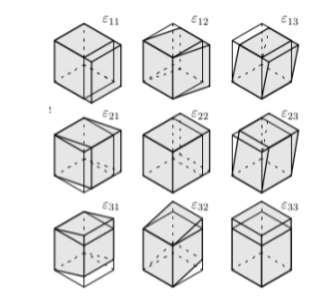
\includegraphics[width = 5cm]{strains1}
	\end{minipage}
	\begin{minipage}{7cm}
		\centering
		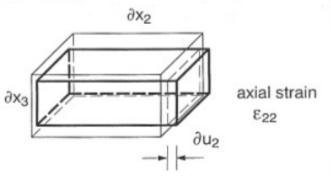
\includegraphics[width = 6cm]{strains2}
	\end{minipage}
	\caption{left: Elongations in different directions, right: elongation in 2-direction (\textit{y-direction})}
	\label{strains}
\end{figure}


\subsection{Constitutive Equations}

Another set of equations are the constitutive equations (CE) which are also referred to as material laws. In mechanics they provide the connection between strains and stresses. 

One example for a CE is Hooke's law which states that the relation between strain and stress in the linear-elastic case is coupled through a stiffness tensor $ \mathbb{C} $. 

\begin{equation}
\vec{\sigma} = \mathbb{C} : \vec{\varepsilon} \qquad \text{or in 1D:} \qquad \sigma = E {\;} \varepsilon
\end{equation}

In 1D the stiffness tensor reduces to the Young's modulus $ E $. 

Hooke's law is one of the easiest CEs that can be applied to a stress-strain-relation. If one also wants to introduce for example plasticity, viscosity or creep the relations become much more complex. 


\subsection{Tonti-Diagram}

The balance equations, kinematic equations and constitutive equations can be summarized in the so-called Tonti-diagram which is shown in figure \ref{tonti1}. 

 
\begin{figure}[h]
	\centering
	\begin{minipage}{10cm}
		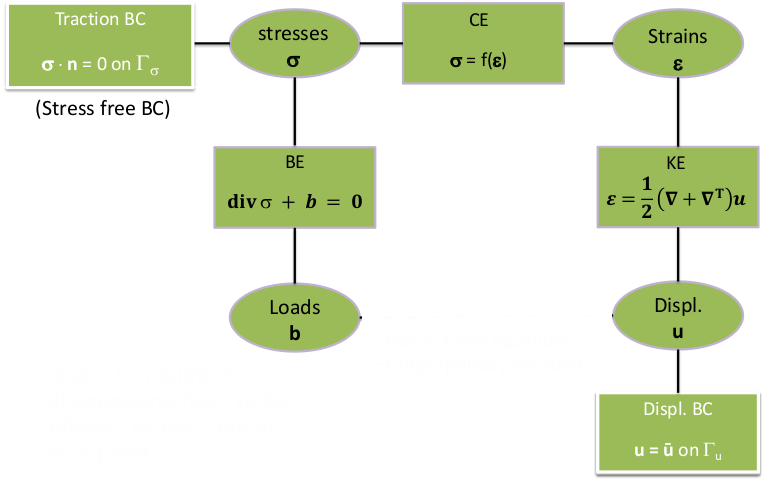
\includegraphics[width = 10cm]{tonti1}
	\end{minipage}
	\caption{The Tonti-diagram}
	\label{tonti1}
\end{figure}

The partial differential equations (PDEs) are obtained through setting up the equations (BEs, CEs and KEs) as a function of the \textit{primary variables}, such as forces and displacements (less frequently as a function of stresses and strains). This will lead to expressions that contain primary variables as well as terms which include derivatives with respect to those (for example equation \eqref{eq12} for the balance of linear momentum).

These PDEs need to be brought into a numerical form for later calculations as pointed out in section 2. 

One example for a PDE is the Navier-Lam�-equation:

\begin{equation}
(\lambda \plus \mu) {\;} \nabla {\;} (\nabla \cdot \vec{u}) \plus \mu {\;} 
\nabla^{2} \vec{u} \plus \vec{F} = 0
\end{equation} 

where $ \lambda $ and $ \mu $ are Lam�-constants, $ \vec{u} $ is the 
displacement field and $ \vec{F} $ are the forces acting on the body. 
However, this formulation is not suitable for finite element applications.  


\subsection{The Weak Form}

A specific treatment of the equations is raised in the concept of FEM. Instead of insisting that all equations need to hold for all points, we just want them to hold in the integral form. 

So, for instance, if there acts a traction force $ \vec{t} $ at the boundary, 
we can put the specific balance equation into a function $ R(x) $.

\begin{equation}
R(x) = \vec{t} - \vec{\sigma} \vec{n} = 0
\end{equation}

The respective integral form is

\begin{equation}
\int R(x) {\;} w(x) \d x ,
\end{equation}

where $ w(x) $ is a weighting function and $ R(x) $ is called 
\textit{residual}. This is why the method is called \textit{method of weighted 
residuals} (MWR). 

The solution for the strong (local) form is automatically also a solution for the weak (global) form. However, for the weak form exist several solutions, and not all of them are solutions for the strong one. 

The MWR is strongly related to the \textit{principle of virtual work} (PVW).

\vspace{0.4cm}


As can be seen in figure \ref{tonti2} the weak formulation is only applied to 
some relations. These are the relations between stress and boundary 
tractions or body forces, respectively. 

 
 \begin{figure}[h]
 	\centering
 	\begin{minipage}{11cm}
 		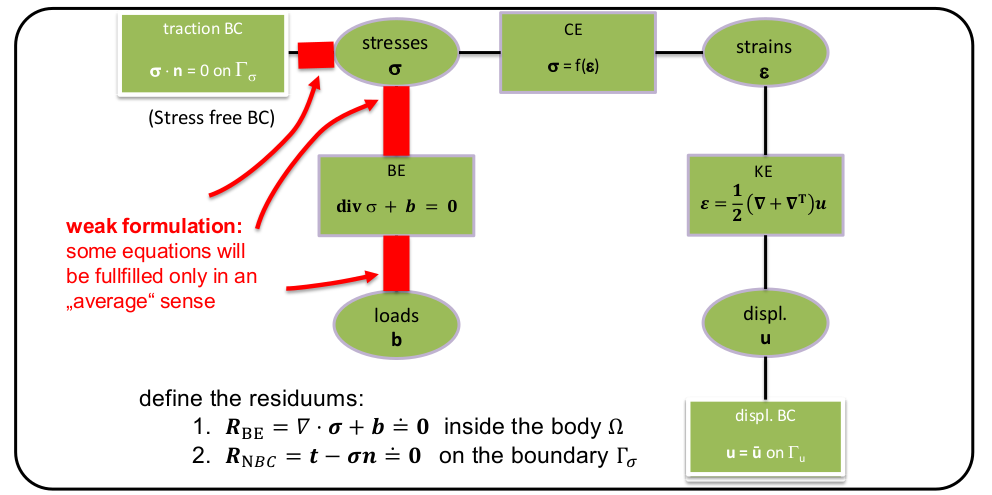
\includegraphics[width = 11cm]{tonti2}
 	\end{minipage}
 	\caption{The Tonti-diagram with the weak formulation}
 	\label{tonti2}
 \end{figure}


The integral formulation for the boundary equation is then 

\begin{equation}
\int\limits_{\Omega} (\vec{t} \minus \vec{\sigma} \vec{n}) \cdot w \d \Gamma \overset{!}{=} 0 .
\end{equation} 

Furthermore, the expression for the body equation follows as

\begin{equation}
\int\limits_{\Omega} (\nabla \cdot \vec{\sigma} \plus \vec{b}) \cdot w \d \Omega \overset{!}{=} 0 , 
\end{equation}

where $ \vec{t} $ and $ \vec{b} $ are the boundary and body forces, respectively. 


\section{Summary}

\begin{multicols}{2}
	\begin{mdframed}
		\textbf{FEM facts} \\
		
		\begin{itemize}
			\item Through the use of flexible elements it is possible to reproduce also \textbf{complex geometries}.
			
			\item The formulation is based on the \textbf{weak form} which only need to be solved in an global sense. 
			
			\item In the \textit{stationary} case only a linear system of equations (LSE) needs to be solved. For \textit{non-stationary} problems also a \textbf{time integration scheme} is necessary.
			
			\item FEM can be used in a huge variety of technical fields: solid mechanics, fluid dynamics, diffusion, etc.
			
			\item One can - depending on the specific problem - use lots of different constitutive equations.
			
			\item The are many commercial (e.g. ABAQUS, COMSOL, MARC) and open source programs available (e.g. feap, deal.ii, libmesh). In general all of them have a \textbf{high level of development}. 
		\end{itemize}
	\end{mdframed}
	
	\begin{mdframed}
		\textbf{Drawbacks} \\
		\begin{itemize}
			\item The mathematical theory behind the method is fairly \textbf{complex}. This is why it is not trivial for all PDEs to implement them into the FEM formulation. 
			
			\item For the computation and the storage of the results a relatively \textbf{high storage capacity} is needed. 
			
			\item The method is very \textbf{error-prone} (e.g. wrong formulation of boundary conditions).
			
			\item If the constitutive equation does not fit the real system, 
			the result is worth nothing. 
			
			\item Some programs - especially commercial ones - tempt the user 
			to execute \textbf{black-box simulations}. If something is wrong, 
			it may be very hard to find the error in this case. (Be aware of 
			that!) 
			
			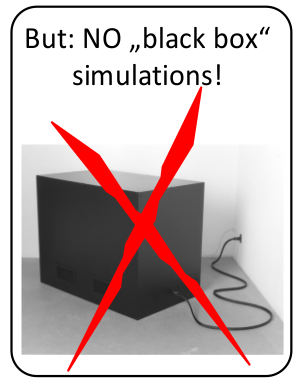
\includegraphics[width=4cm]{blackbox}
		\end{itemize}
	\end{mdframed}
	
	
	
	
	
	
\end{multicols}




































	
\end{document}